% chktex-file 46
\pagebreak
\section{Theory}\label{sec:theory}
We present our theoretical results in this section.
We use the work of \cite{chitra20analyzing}
as a foundation for our results.

We consider the Stochastic Block Model (SBM)
with two blocks each of size $n$ where the probability
of an edge between nodes in the same block is $p$
and the probability of an edge between nodes in different
blocks is $q$.

\subsection{Equilibrium in Expectation}
We first analyze the expected SBM.
In this subsection, we do not require any bounds on $p$ and $q$
besides $0 \leq p,q \leq 1$ to ensure both are valid probabilities. Our first result is that we can express the equilibrium vector, $z^*$ as a linear combination of \emph{any} mean-centered opinion vector, rather than simply the innate opinion vector $s$
(as in \cite{chitra20analyzing}).

\begin{theorem}\label{thm:expectz}
Let $\bar{G}$ be the expected SBM graph with $2n$ nodes
and adjacency matrix $\bar{A}$ where

\begin{figure}[h]
    \centering
    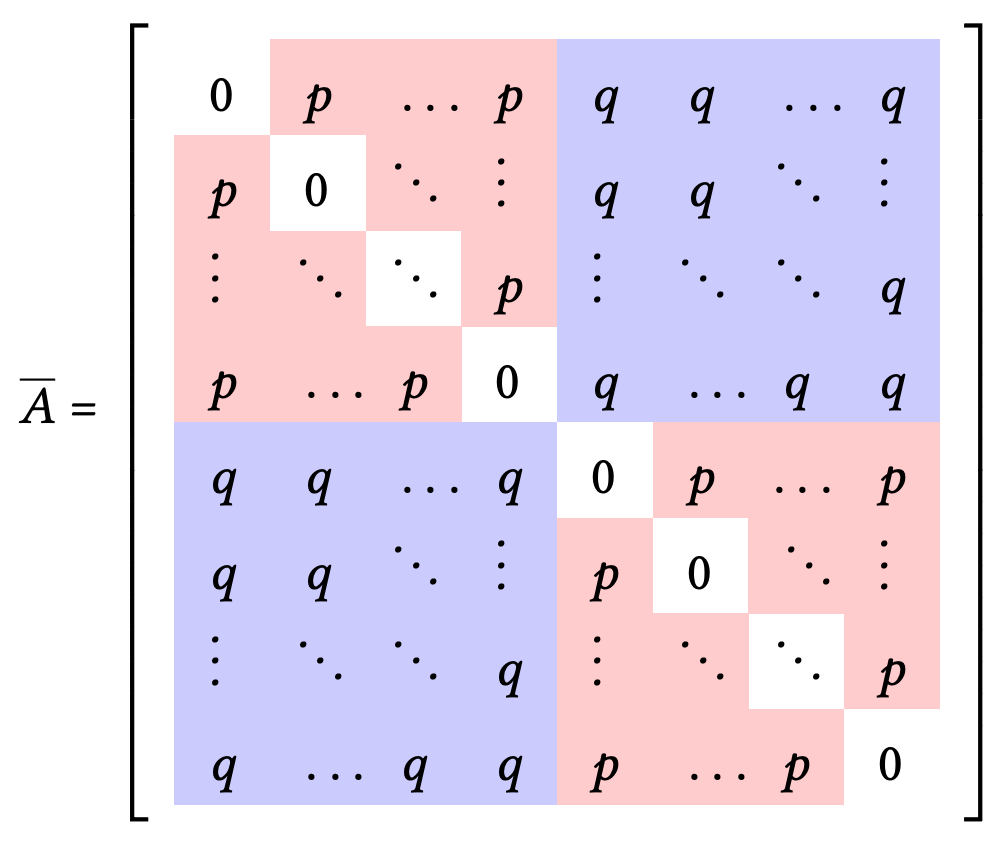
\includegraphics[scale=.2]{expectedA.png}
\end{figure}

Let $s$ be any mean-centered innate opinion vector
and let $z^*$ be the resulting equilibrium opinion
vector according to FJ dynamics.
Recall $z^* = (\bar{L}+I)^{-1}s$ where $\bar{L}$
is the Laplacian of $\bar{G}$.
Let $(\bar{L}+I)=\bar{U}\bar{S}\bar{U}$ where
$\bar{U}$ and $\bar{S}$ the eigendecomposition defined below.
Then
\begin{align}
    z^* = \frac{c_2}{2nq + 1} u^{(2)}
    + \frac{c_3}{nq +np + 1} u^{(3)}
    + \cdots + \frac{c_3}{nq +np + 1}u^{(3)} \nonumber
\end{align}
where $u^{(i)}$ is an eigenvector of $(\bar{L}+I)$ for
$i \in \{2, \ldots, 2n\}$.

\end{theorem}
\begin{proof}
Let $U' = \begin{bmatrix} u^{(1)} & u^{(2)} \end{bmatrix}$
where $u^{(1)}$
is the normalized all 1's vector and $u^{(2)}$
is the normalized vector with $n$ 1's followed
by $n$ -1's.
A back-of-the-envelope calculation shows that
$\bar{A} + p I=U'S'U'^T$
where $S' = \textrm{diag}(np+nq, np-nq)$.
Now, define $\bar{U} = \begin{bmatrix} u^{(1)} & u^{(2)} 
& Z \end{bmatrix}$,
where $Z \in \R^{2n \times (2n-2)}$ is a matrix
with orthonormal columns satisfying
$Z^T u^{(1)} = 0 = Z^T u^{(2)}$ built by
extending $u^{(1)}$ and $u^{(2)}$ to an orthonormal
basis.

With the observation that $\bar{U}\bar{U}^T
= \bar{U}^T \bar{U} = I$, we have:
\begin{align}\label{eq:decomposeLI}
    \bar{L}+I &= \bar{D} + I - \bar{A}
    = (np + nq)I + I - (\bar{A} + pI)
    \nonumber \\
    &= (np + nq + 1)I - U'S'U'^T
    = \bar{U}\bar{S}\bar{U}^T
\end{align}
where $\bar{S}=\textrm{diag}
(1, 2nq+1, np+nq+1, \ldots, np+nq+1)$.
Since $\bar{U}$ is an orthonormal basis, it follows that
$(\bar{L}+I)^{-1} = \bar{U}\bar{S}^{-1}\bar{U}$.
Additionally, because $\bar{U}$ is an orthonormal basis,
we can write: 
\begin{align}
    s = c_1 u^{(1)} + c_2 u^{(2)} 
    + \cdots + c_{2n} u^{(2n)}
    \nonumber
\end{align}
for scalars $c_i \in \R$
and columns $u^{(i)}$ of $\bar{U}$ 
where $i \in [2n]$.
Notice that $c_1 =0$ since $s$ is mean-centered.
Then we have that:
\begin{align}
    z^* = (\bar{L}+I)^{-1} s &= \bar{U}\bar{S}\bar{U}^T
    (c_2 u^{(2)} + c_3 u^{(3)} + \cdots + c_{2n} u^{(2n)})
    \nonumber \\
    &= \bar{U}\bar{S} \begin{bmatrix}
        0 & c_2 & c_3 & \cdots & c_{2n}
    \end{bmatrix}^T \nonumber \\
    &= \frac{c_2}{2nq + 1} u^{(2)}
    + \frac{c_3}{nq +np + 1} u^{(3)}
    + \cdots + \frac{c_3}{nq +np + 1}u^{(3)} \nonumber
\end{align}

\cref{thm:expectz} immediately follows.
\end{proof}

\subsection{Polarization Bounds}
We next present bounds for the polarization of the equilibrium
opinion resulting from FJ dynamics on any mean-centered
innate opinion vector. We extend the results of \cite{chitra20analyzing}
in the following ways:
\begin{itemize}
  \item Instead of requiring innate opinion vectors where the first block
  has opinion all 1 and the second block has opinion all -1,
  we allow for any mean-centered innate opinion vector.
  \item We consider the additional case of $q \geq p$. This case has real-world applications: for example, when dealing with opinion formation in a network of doctors and patients, opinions may be more likely to develop between doctors and patients
  than doctors and doctors or patients and patients.
  \item We explicitly describe the factors on the bound
  of polarization, and explain how they tighten as $n$ increases.
  \item We describe the special case $p=q$, equivalent to
  the Erdős-Rényi graph, and tightly characterize the bounds
  in this case.
\end{itemize}
Unfortunately, we trade the extension to any mean-centered
innate opinion to a limited result.
Instead of allowing $q \geq 1/n$, as in \cite{chitra20analyzing},
we require $q \geq p/2$.

\begin{theorem}\label{thm:converge}
  Let $G$ be a graph generated by the Stochastic Block Model
  with $p/2 \leq q \leq p$ and $p \geq C \log^4n/n$ or
  with $1/n \leq p \leq q$ and $q \geq C \log^4n/n$
  for some universal constant $C$.
  Let $s$ be any mean-centered innate opinion vector
  on $2n$ nodes and let $z^*$ be the equilibrium opinion
  vector according to FJ dynamics.
  Then for sufficiently large $n$,
  \begin{align}
    C' \frac{||s||_2^2}{(2nq+1)^2} \leq \Pz \leq
    C'' \frac{||s||_2^2}{(2nq+1)^2}
    \nonumber
  \end{align}
  with probability 97/100 where $C' \geq 1/6$
  and approaches $1/2$ as $n$ grows while
  $C'' \leq 16$ and approaches $4$ as $n$ grows.
\end{theorem}

\begin{proof}
At a high level, we prove \cref{thm:converge}
by writing $\Pz = s^T(L+I)^{-2}s$ 
and bounding the eigenvalues of $(L+I)^{-2}$
through clever comparisons to $\bar{L}$,
where $L$ is the Laplacian of $G$
and $\bar{L}$ is the Laplacian of the expected SBM $\bar{G}$.

First, notice that the normalized all 1's vector
$u^{(1)}$ is an eigenvector
of $(\bar{L}+I)$ by \cref{eq:decomposeLI}; $u^{(1)}$ is also an eigenvector
of $(L+I)$, since the columns and rows of $L$
must sum to 0 (by the definition of a graph Laplacian).
Unfortunately, $u^{(1)}$ has eigenvalue 1
for both $(L+I)^{-2}$ and $(\bar{L}+I)^{-2}$,
which poses a problem for the
bound we want to achieve.
We deal with this by
observing that $s$ is mean-centered and so
does not have any scaling of $u^{(1)}$.
It follows that
\begin{align}
    \Pz = s^T (L+I)^{-2} s = s^T (I-P)
    (L+I)^{-2}(I-P) s \nonumber
\end{align}
where $P$ is the projection $u^{(1)} {u^{(1)}}^T$.
The point of $(I-P)$ is to remove the eigenvector $u^{(1)}$
and corresponding eigenvalue 1.
Therefore, to bound $\Pz$, it is sufficient to
bound the eigenvalues of $(I-P)(L+I)(I-P)$, since
$s$ is some linear combination of the eigenvectors of
$(I-P)(L+I)(I-P)$.
To bound the eigenvalues of $(I-P)(L+I)(I-P)$,
we use \cref{lemma:boundL}, which tells us that the
eigenvalues of $L$ and $\bar{L}$ are within
$.5n\Mpq$ of each other for sufficiently large $n$.
We leave the proof of \cref{lemma:boundL} to
\cref{app:proof} for brevity.

\begin{lemma}[Extension of Lemma 4.5 in \cite{chitra20analyzing}]\label{lemma:boundL}
    Let $L$ be the Laplacian of graph $G$ drawn from
    the SBM and let $\bar{L} =\E[L]$. For fixed constant
    $C'$, with probability 98/100,
    \begin{align}
        ||L - \bar{L}||_2 \leq C' \sqrt{ n \log n \Mpq} \nonumber.
    \end{align}
\end{lemma}

Note that when $\Mpq \geq C \log^4 n /n$,
$C' \sqrt{ n \log n \Mpq} \leq \frac{C'}{\sqrt{C} \log^{1.5} n}
n \Mpq$.
So for $n \geq \exp(\frac{C'}{\sqrt{C}\epsilon})^{2/3}$,
$||L-\bar{L}||_2 \leq \epsilon n \Mpq$.
Choose $\epsilon = 1/2$.

From Weyl's Inequality and \cref{lemma:boundL}, we now have that
\begin{align}\label{eq:weyls}
    |\lambda_i - \bar{\lambda}_i| \leq ||L - \bar{L}||_2 \leq 
    \frac{1}{2} n \Mpq
\end{align}
for sufficiently large $n$,
where $\lambda_i$ is the $i$th eigenvalue of $L$ and 
$\bar{\lambda}_i$ is the $i$th eigenvalue of $\bar{L}$.
We now bound the largest $2n-1$ eigenvalues of $L+I$
or, equivalently, the eigenvalues of $(I-P)(L+I)(I-P)$.
The eigenvalues of $(I-P)(\bar{L}+I)(I-P)$ are $2nq+1$
and $np+nq+1$.

\paragraph{Case 1: \boldmath$q \geq p$}
The smallest eigenvalue of $(I-P)(\bar{L}+1)(I-P)$
is $nq+np+1 \geq nq+1$ while the largest eigenvalue is $2nq+1$.
Then, \cref{eq:weyls} implies that:
\begin{align}
    (.5nq + 1)(I-P)\preceq(I-P)(L+I)(I-P)\preceq(2.5nq+1)(I-P)
    \nonumber.
\end{align}
We square and invert each term, which yields:
\begin{align}
    (2.5nq + 1)^{-2}(I-P)\preceq(I-P)(L+I)^{-2}(I-P)
    \preceq(.5nq+1)^{-2}(I-P).
    \nonumber
\end{align}
Now, we can bound
\begin{align}
    \frac{1}{2} \frac{||s||_2^2}{(2nq+1)^2}
    \leq \frac{||s||_2^2}{(2.5nq+1)^2}
    \leq s^T(L+I)^{-2}s
    \leq \frac{||s||_2^2}{(.5nq+1)^2}
    \leq \frac{16||s||_2^2}{(2nq+1)^2}.
    \nonumber
\end{align}

\paragraph{Case 2: \boldmath$p \geq q \geq p/2$}
The smallest eigenvalue of 
$(I-P)(L+I)(I-P)$ is $2nq+1 \geq np+1$
while the largest eigenvalue is $nq+np+1 \leq 2np+1$.
Similar analysis to Case 1 yields
\begin{align}
    \frac{1}{6}\frac{||s||_2^2}{(2nq+1)^2}
    \leq \frac{||s||_2^2}{(2.5np+1)^2}
    \leq s^T(L+I)^{-2}s
    \leq \frac{||s||_2^2}{(.5np+1)^2}
    \leq \frac{16||s||_2^2}{(2nq+1)^2}.
    \nonumber
\end{align}
We now justify the
upper and lower bound on $C'$
and $C''$, respectively.
Consider a small $\epsilon$ such that
\cref{lemma:boundL} gives a small additive error.
Then, without loss of generality, the largest eigenvalue between Cases 1 and 2
is $(2+\epsilon)np+1$.
It follows that $C'$ gets arbitrarily close to $1/2$
as $n$ grows.
The smallest eigenvalue between Cases 1 and 2
$(1-\epsilon)np+1$ without loss of generality.
It follows that $C''$ gets arbitrarily close $4$
as $n$ grows.
\end{proof}

%\cref{thm:converge} applies to the SBM,
For $p=q$, the SBM
is simply an Erdős-Rényi random graph.
Therefore, a special case follows immediately
from \cref{thm:converge}.

\begin{theorem}[Erdős-Rényi Special Case]
    Let $G$ be a Erdős-Rényi graph where
    the probability of an edge between any pair
    of nodes is $p \geq C \log^4 n/n$ for some
    universal constant $C$.
    Let $s$ be any mean-centered innate opinion
    vector on $2n$ nodes
    and let $z^*$ be the equilibrium opinion vector
    according to $FJ$ dynamics.
    Then for sufficiently large $n$,
    \begin{align}
        C' \frac{||s||_2^2}{(2np+1)^2} \leq \Pz \leq
        C'' \frac{||s||_2^2}{(2np+1)^2}
        \nonumber
    \end{align}
    with probability 97/100 where $C' \geq 1/2$
    and $C'' \leq 2$. Both $C'$ and $C''$ approach
    1 as $n$ increases.
\end{theorem}

\begin{proof}
    The theorem immediately follows as a
    special case of \cref{thm:converge},
    except for the improved constants $C'$ and $C''$.
    To obtain the improved bounds, observe that
    the only eigenvalue of $(I-P)(L+I)(I-P)$
    is $2np+1$.
    Then, following the earlier analysis, we have that:
    \begin{align}
        \frac{1}{2}\frac{||s||_2^2}{(2np+1)^2}
        \leq \frac{||s||_2^2}{(2.5np+1)^2}
        \leq s^T(L+I)^{-2}s
        \leq \frac{||s||_2^2}{(1.5np+1)^2}
        \leq \frac{2||s||_2^2}{(2np+1)^2}.
        \nonumber
    \end{align}
    Setting $\epsilon$ to a small positive value
    yields an upper bound of $(2+\epsilon)np+1$
    on the eigenvalues and a lower bound
    of $(2-\epsilon)np+1$.
    It is easy to see that the factors
    $C'$ and $C''$ get arbitrarily close to 1
    as $\epsilon$ decreases.
    
\end{proof}

We remark that extending our results to the case of
$1/n \leq q \leq p/2$
would require bounding the inner product of the
largest $n-2$ eigenvectors, even if the innate opinion
vector $s$ did not have any scaling of the all 1's
vector or the second smallest eigenvector.


